\documentclass[12pt,letterpaper,final,oneside,openany,onecolumn]{book} 												
\usepackage[lmargin=3.5cm,rmargin=2.5cm,tmargin=3.0cm,bmargin=3.0cm]{geometry}
\usepackage[latin1]{inputenc}												%european 
\usepackage[T1]{fontenc}
\usepackage[]{times}
\usepackage[spanish]{babel}													%espa�ol
\usepackage{amsmath}																%math package
\usepackage{graphicx}
\usepackage{multicol}
\usepackage{url}
\usepackage{amssymb}
\usepackage{array}
\usepackage{algorithm_spa}
\usepackage{algpseudocode}
\usepackage[footnotesize]{subfigure}
\usepackage{makeidx}
\usepackage{color}
\makeindex
%\renewcommand{\baselinestretch}{1}
%\renewcommand{\contentsname}{�ndice General}%{Tabla de Contenidos}
%\renewcommand{\listfigurename}{Lista de Figuras}
%\renewcommand{\listtablename}{\'Indice de Tablas}
%\renewcommand{\chaptername}{Cap�tulo}
%\renewcommand{\bibname}{Bibliograf�a}
\renewcommand\floatpagefraction{.9}
\renewcommand\topfraction{.9}
\renewcommand\bottomfraction{.9}
\renewcommand\textfraction{.1}
\addto\captionsspanish{%
  \renewcommand{\tablename}%
    {Tabla}%
}

\setcounter{totalnumber}{50}
\setcounter{topnumber}{50}
\setcounter{bottomnumber}{50}

% Different font in captions
\newcommand{\captionfonts}{\small}

\makeatletter  % Allow the use of @ in command names
\long\def\@makecaption#1#2{%
  \vskip\abovecaptionskip
  \sbox\@tempboxa{{\captionfonts #1: #2}}%
  \ifdim \wd\@tempboxa >\hsize
    {\captionfonts #1: #2\par}
  \else
    \hbox to\hsize{\hfil\box\@tempboxa\hfil}%
  \fi
  \vskip\belowcaptionskip}
\makeatother   % Cancel the effect of \makeatletter

%Inicio de documento
\begin{document}
\hyphenation{pa-la-bra}

\renewcommand{\contentsname}{Tabla de Contenidos}
%\renewcommand{\listfigurename}{Lista de Figuras}
%\renewcommand{\listtablename}{Lista de Tablas}
	\frontmatter
		\label{ch:portada}
\thispagestyle{empty}

%\vspace{-2.0cm}
	\begin{figure}[t]
						\centering
							\includegraphics[height=0.15\textwidth]{./images/logoUCV.jpg}
	\end{figure}
					\begin{center}
						Universidad Central de Venezuela\\
						Facultad de Ciencias\\
						Escuela de Computaci\'on\\
						Centro de Computaci\'on Gr\'afica\\
					\end{center}
					
					\vspace{2.5cm}
					\begin{center}
						\large{\textbf{T\'itulo de la tesis}}
					\end{center}
					
					\vspace{5.2cm}
					\begin{center}
						Trabajo Especial de Grado \\
						presentado ante la Ilustre\\
						Universidad Central de Venezuela\\
						Por el (o los) Bachiller (es)\\
						Mark Hamill\\
						para optar el t�tulo de \\
						Licenciado en Computaci\'on
					\end{center}
					
					\begin{center}
						Tutor: Prof. Luke Skywalker\\
					\end{center}
					
					\vspace{1.0cm}
					\begin{center}
						Caracas, Diciembre de 2020
					\end{center}
						
					
%\newpage
		%\input{agradecimientos}	%opcional
		%\input{dedicatoria}		%opcional
		\chapter*{Resumen}

Esbozo sucinto del contenido del TEG, presentando objetivos, resultados y conclusiones (m\'aximo media p\'agina). \\


\noindent \textbf{Palabras Claves}: palabra1, palabra2, palabra3, palabra4, palabra5
		\tableofcontents	%indice
		\listoffigures	%opcional
		\listoftables		%opcional
		\chapter{Introducci\'on}

Es una introducci\'on al TEG como documento y no al tema mismo, de modo que oriente al lector. Se recomienda incluir los siguientes aspectos:
\begin{itemize}
	\item Motivaciones para hacer el Trabajo.
	\item Objetivos que persigue el Trabajo.	
	\item Descripci\'on del contenido de los diferentes cap\'itulos del TEG
\end{itemize}
	\mainmatter
		\chapter{Marco Te\'orico}

%%%%%%%%%%%%%%%
%%%%%%%%%%%%%%%
\section{first}

%%%%%%%%%%%%%%%
\subsection{first-1}
Esto es un ejemplo de referencia \cite{STRO01}. Esto es un ejemplo de c\'odigo en pseudoformal:


\begin{algorithmic}[upquote=true, language=pseudo]
	\Require $n \geq 0$
	\Ensure $y = x^n$
	\State $y \Leftarrow 1$
	\State $X \Leftarrow x$
	\State $N \Leftarrow n$
	\While{$N \neq 0$}
	\If{$N$ is even}
	\State $X \Leftarrow X \times X$
	\State $N \Leftarrow \frac{N}{2} $  \Comment{This is a comment}
	\ElsIf{$N$ is odd}
	\State $y \Leftarrow y \times X$
	\State $N \Leftarrow N - 1$
	\EndIf
	\EndWhile
\end{algorithmic}
%%%%%%%%%%%%%%%
%%%%%%%%%%%%%%%
\section{second}

Las tablas, se pueden hacer con \url{https://www.tablesgenerator.com} y referenciarlos \ref{lb:table1}.

\begin{table}[htpb!]
	\centering
	\begin{tabular}{ll}
		Value & Description         \\
		3     & None to say         \\
		2     & Fill with something
	\end{tabular}
	\caption{Irrelevant data}
	\label{lb:table1}
\end{table}

%%%%%%%%%%%%%%%
\subsection{second-1}
Las referencias tambi\'en pueden hacerse en conjunto \cite{REF_MIC,WEB99}.



\noindent Aqu\'i las otras referencias \cite{RAM11}

\subsubsection{second-1-1}

Para insertar im\'agenes, hay diversos enfoques (incluyendo subfigure) \ref{fig:reloj}.

\begin{figure}[htpb!]
	\centering
	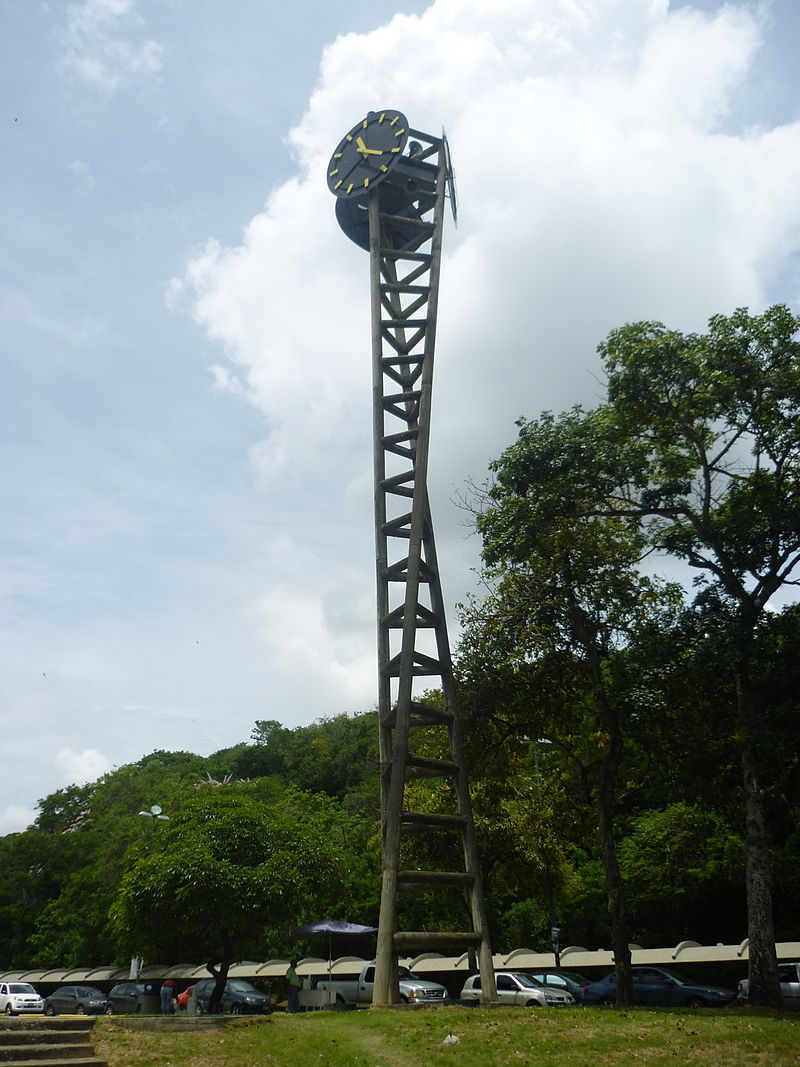
\includegraphics[width=0.5\columnwidth]{images/reloj.jpg}
	\label{fig:reloj}
	\caption{Reloj sin chichero}
\end{figure}


		%\input{chapter2}
		%\input{chapter3}
		%\input{chapter4}
		%\input{chaptern}
		\chapter{Conclusiones y Trabajos futuros}

%%%%%%%%%%%%%%%%%%%%%%%%%%%%%%%%%%%%%%%%%%%%%%%%
\section{Conclusiones}

Evaluar\'a los resultados obtenidos y la metodolog\'ia y herramientas utilizadas. Determinar si se lograron los resultados esperados y, si as\'i no fuera, explicar las razones, donde se incluye la soluci\'on lograda del problema; emitir juicio objetivo sobre las actividades y tareas cumplidas, importancia del aporte, sugerencias, etc.

%%%%%%%%%%%%%%%%%%%%%%%%%%%%%%%%%%%%%%%%%%%%%%%%
\section{Trabajos futuros}

Que recomendaciones, sugerencias y futuros aporte considera para mejorar el trabajo actual de manera significativa.
	\backmatter
		\bibliographystyle{IEEEtran}
		%\bibliographystyle{plain}     %You may prefer \bibliographystyle{alpha}
		%\bibliographystyle{alpha}
		%\bibliographystyle{babalpha}
		\bibliography{books}
		\nocite{*}
		\chapter{Anexos}

%%%%%%%%%%%%%%%%%%%%%%%%%%%%%%%%%%%%%%%%%%%%%%%%
Documentos, tablas, cronogramas, c\'alculos, planos etc. que dificulten la lectura del informe y que han sido citados en \'este. Agregar \# c\'odigo fuente	%opcional
\end{document}